\chapter{Installation}

\section{Prerequisites}

\begin{itemize}
\item This package aims at automating GSAS, therefore, a running GSAS is required. To test this, at the command line from which you wish to run this (mouse junkies - this will NOT be your cup of tea - but maybe we can pull you into the great land of command lines) change into a folder with GSAS data and try to plot it in rawplot by typing in \texttt{rawplot}. If this fails with a file not found error, GSAS is either not installed or not in the search path\footnote{On windows systems, go to the control panel, advanced setup, environment variables, and add "\texttt{;c:\textbackslash gsas\textbackslash exe}" at the end of the search path. On Unix systems, add ":/usr/local/gsas/exe" to you PATH variable in something like \texttt{\textasciitilde/.bashrc} or so.}. If it plots, but doesn't have text around the graph, the PGPLOT\_FONT variable is not set. Another missing bit could be the GSAS variable, in which case GSAS wouldn't know where to look for the scattering length etc. All this is documented somewhat in the README file coming with GSAS, but who reads those these days... Please note that PC-GSAS and EXPGUI are setting the environment variables only for the current session, that is not enough for what we want to do here, so a running PC-GSAS or EXPGUI is not sufficient.
\item The 2nd prerequisite is a working understanding of GSAS by the user. If you don't know what GSAS does and how it works, automation will be of little help, it might be even dangerous due to the GIGO problem\footnote{garbage in, garbage out}... We strongly suggest you work at least through the excellent tutorials that come with GSAS to get an idea what GSAS does. To encourage that, the examples we provide here are the tutorials from the GSAS manual cast into scripts.
\end{itemize}

\section{GSAS installation}

The best starting point to install GSAS and EXPGUI is \url{https://subversion.xor.aps.anl.gov/trac/EXPGUI/}. From there, go to the "New installation instructions" for your operating system. In order to use the subversion automatic update and installation mode, on Unix systems you may have to add the lines

\texttt{\\
http-proxy-host = proxyout.lanl.gov\\
http-proxy-port = 8080\\
}

into the subversion server configuration stored in \texttt{~/.subversion/servers}. Otherwise you will get an error message that subversion could not connect to the server at APS.


\section{Linux or Windows?}

We found that the same stuff runs faster when a given system runs under Linux. Here are some numbers on a 28 histogram refinement, including 8th order spherical harmonics texture. On both platforms, the same data was analyzed with the same script. The platform was a Dell Optiplex 960 (Quadcore Intel CPU, 3GHz, 4GB RAM). No other major tasks were running on the machine.

\begin{tabular}{|l|c|c|}
\hline
&Linux&Windows\\
\hline
OS&OpenSuse&Windows XP Professional\\
Version&11.2, Kernel 2.6.31.14-0.6 SMP&5.1.2600 SP3 Build 2600\\
total runtime [s]&2497&2652\\
average GENLES cycle time [s]&11.2(2.7)&12.4 (3.2)\\
Minimum GENLES cycle time [s]&4.1&4.8\\
Maximum GENLES cycle time [s]&18.5&20.1\\
\hline
\end{tabular}

On average, each GENLES cycle is 9\% faster when running Linux with a maximum improvement of 17\%. The overall runtime is reduced by 6.2\% when running Linux.

\section{Linux/Mac/Unix Installation}
This should be fairly quick:
\begin{itemize}
\item Download the zip file with the latest scripts from \url{http://code.google.com/p/gsaslanguage/}. 
\item Copy the scripts into an appropriate folder and add it to the path\footnote{Add something like\newline \texttt{PATH=\$PATH:/usr/local/gsas/exe:$\sim$/gsaslanguage\newline export PATH\newline} to your \texttt{~/.bashrc} file if you installed GSAS in \texttt{/usr/local/gsas} and gsaslanguage in a folder of the same name in your home folder, adapt as needed by your installation. If you are there, also add \texttt{\\export GSAS=/usr/local/gsas \\export PGPLOT\_FONT=\$GSAS/pgl/grfont.dat}.Run \texttt{source $\sim$/.bashrc} to activate your changes for the current shell, new shells will read it from the \texttt{$\sim$/.bashrc} file. Try \texttt{echo \$PATH} to see if it was added.}. Done.
\item If you want to get the very latest version and you have subversion
installed on your system, navigate to the folder under which you want
gsaslanguage installed, and type\\
\texttt{svn checkout https://gsaslanguage.googlecode.com/svn/trunk/
gsaslanguage}
\item Ok, maybe not completely. Make sure you have \LaTeX{}  installed (punch in \texttt{latex} at a command prompt, it should come up with a \LaTeX{}  prompt). If you want to plot the results of a multi-run analysis using gsas\_plot\_overview, make sure you have gnuplot installed, try typing \texttt{gnuplot} at a shell prompt.
\end{itemize}

\section{Windows Installation}

This is a bit more lengthy since many of the Unix standard software, like a bash shell, \LaTeX{}  and gnuplot don't come with the standard Windows.
\begin{itemize}
\item Copy the scripts into an appropriate folder, e.g. \texttt{c:\textbackslash gsaslanguage} 
\item Since we need a bash shell, install the cygwin package from (www.cygwin.com).  Download the setup executable and store it in the same folder where you will install cygwin (e.g. \texttt{c:\textbackslash cygwin} ). That way it can be used for future additions and updates. Provide your internet options. If you are working at a U.S. government lab, choose a cygwin site at another government lab (.gov) since they are connected with a high-speed backbone. Once you see the ``select packages'' screen (see screenshot below), click on the ``View'' button in the top right corner until you see the ``Full'' view. Besides the basic cygwin, select to install also gnuplot and bc.  Make sure to follow the UNIX end-of-line convention, if in doubt (getting weird error messages when running the gsas scripts such as ``unexpected end of file'' or so), run ``dos2unix'' on your script from the command line.
\begin{figure}[h]
\centering
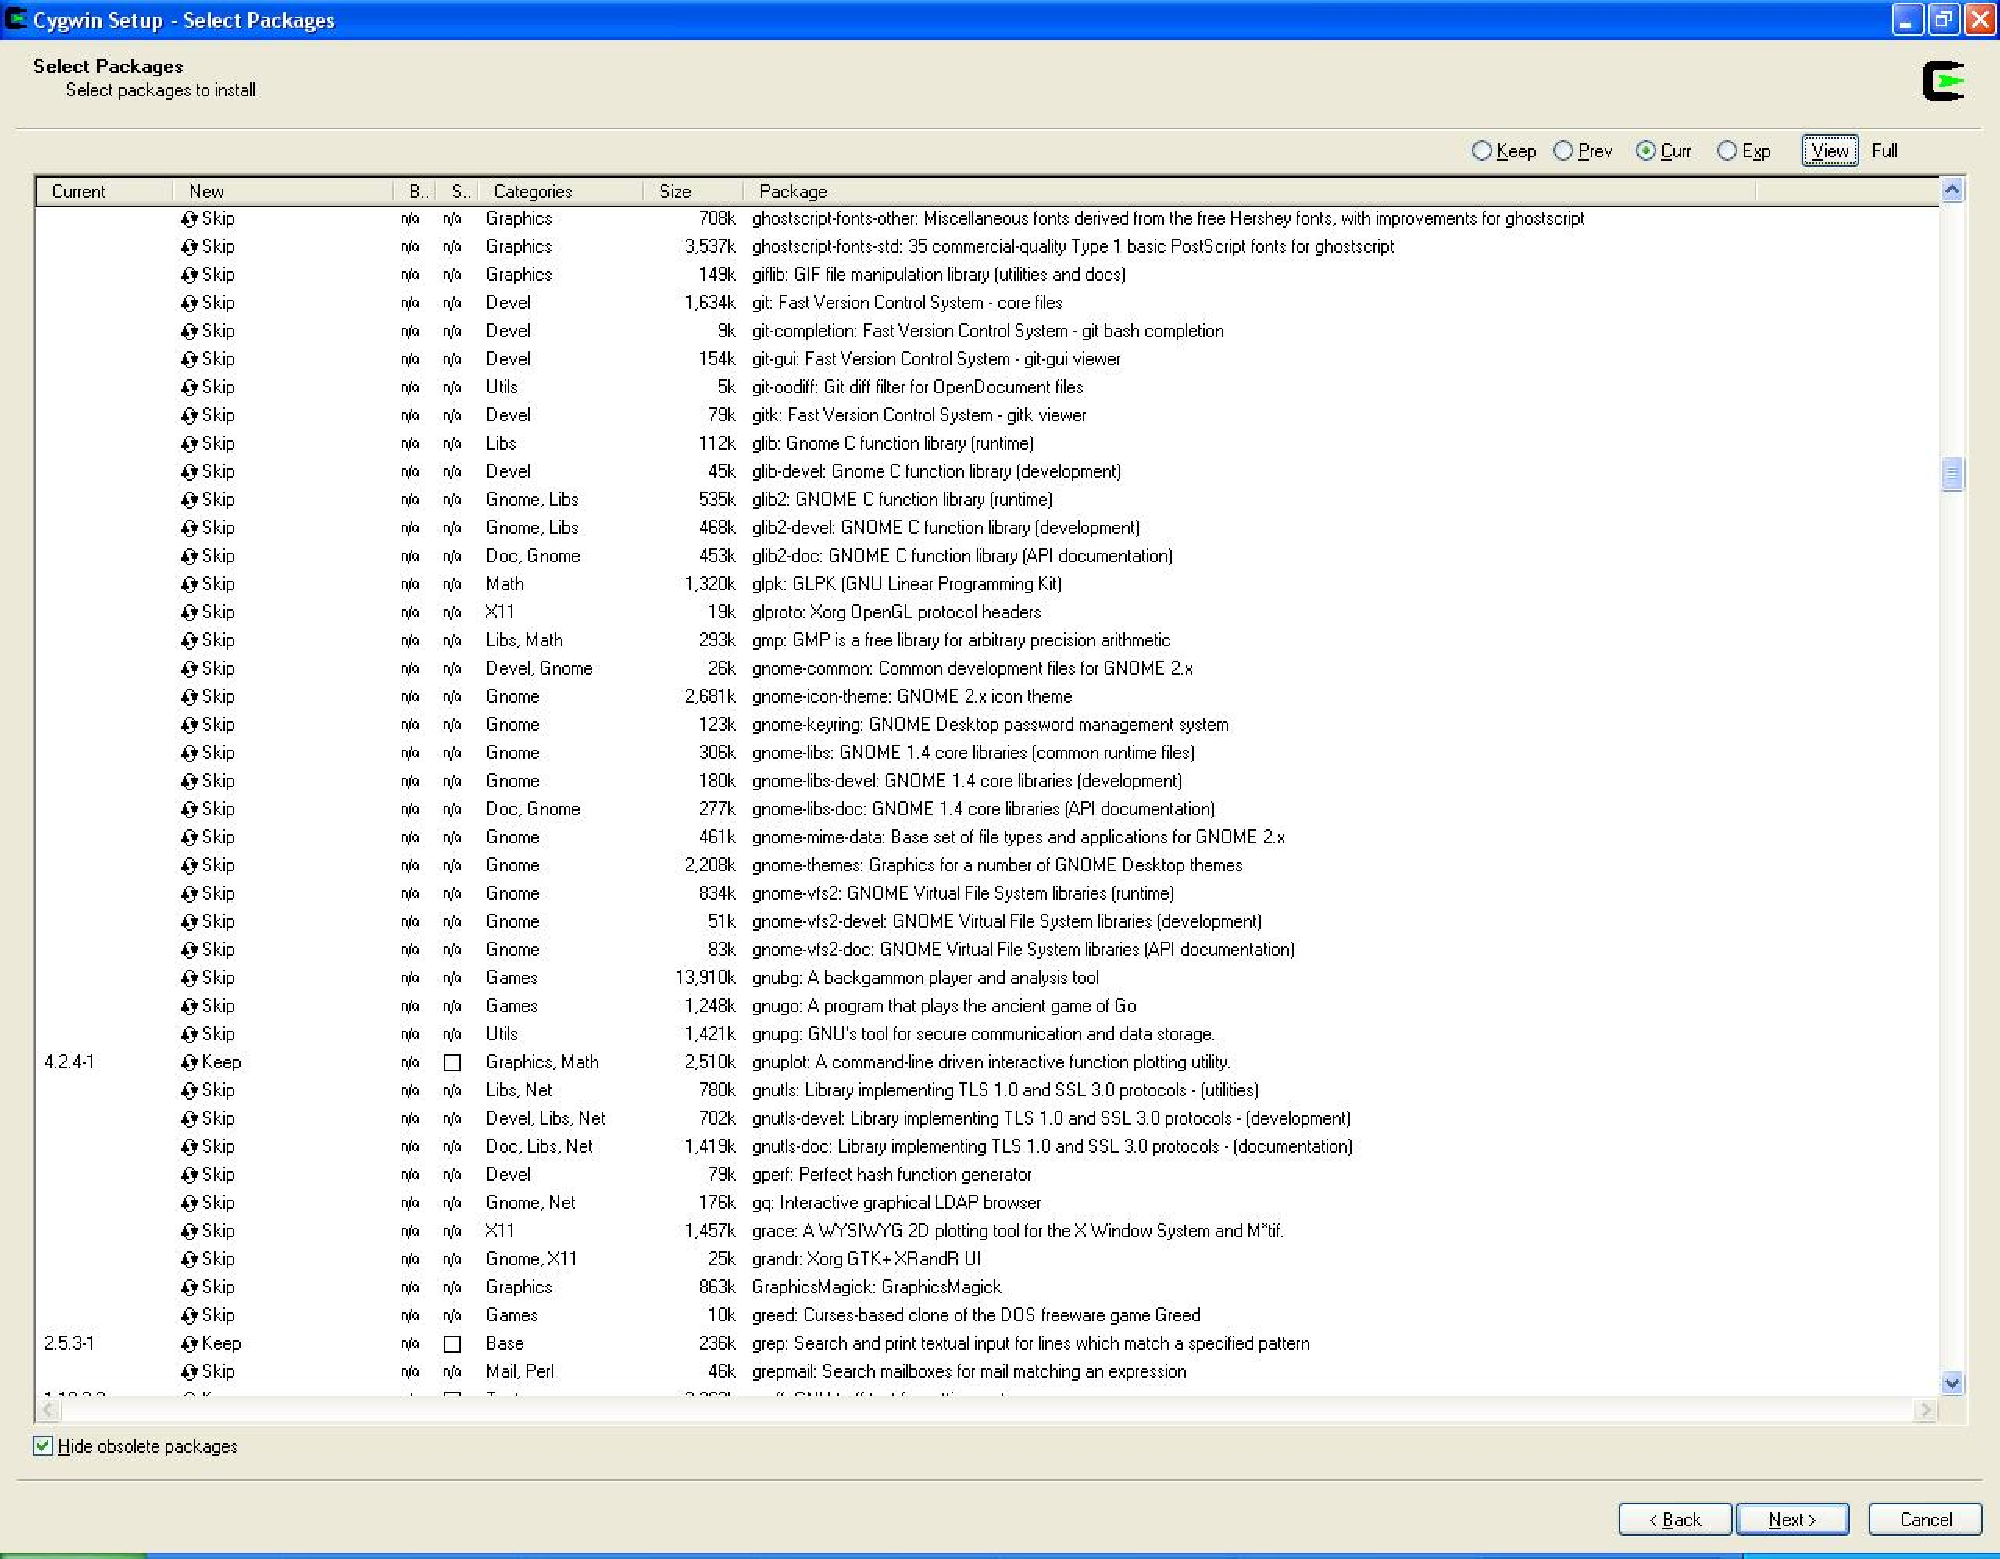
\includegraphics[width=12cm]{Screenshot1.pdf}
\caption{Selecting packages during Cygwin installation}
\label{fig:Screenshot1}
\end{figure}

\item Get the GSAS scripts from \url{http://code.google.com/p/gsaslanguage/}. Add the folder name to the search path (Control Panel -- System -- Advanced
-- Environment Variables -- PATH)
\item Install \LaTeX{}  (go to miktex.org to download the basic installation for a Windows system).
\item You may have to install the \LaTeX{}  package fullpage manually if your firewall does not allow \LaTeX{}  to install it on the fly. If you are using Miktex (Basic MiKtex 2.7), install it into a subfolder of your Miktex installation and refresh the Filename database in the Miktex options.
\end{itemize}

\section{Testing an Installation}
On all platforms it's worth to try a few things to be sure GSAS and other programs are installed correctly before executing scripts. Try these:
\begin{itemize}
\item Type \texttt{expedt} and hit enter. EXPEDT should ask "Enter the experiment name for EXPEDT >". Hit Ctrl-c to exit. If this does not work, either GSAS is not installed or the GSAS executables are not in the search path.
\item Change to the folder with the GSAS demo data by typing "cd \$GSAS/example". If you get a message like "no such file or directory", your GSAS variable was not set properly. Try \texttt{echo \$GSAS} to see if it points to the GSAS folder.
\item If you got there, list the files in there by typing \texttt{ls} followed by enter.
\item Go back to your home folder by typing \texttt{cd} followed by enter. Start RAWPLOT by typing \texttt{rawplot} followed by enter. Select a suitable screen option (a on Linux, c on Windows), take the default of the next question, load the \texttt{nickel.raw} file from the previous folder, e.g. type \texttt{\\/usr/local/gsas/example/nickel.raw\\}. Take the default of the next question by hitting enter, load the \texttt{inst\_tof.prm} instrument parameter file by typing \texttt{\\/usr/local/gsas/example/inst\_tof.prm\\} Type \texttt{b 1 p} followed by enter. If you don't see graphics, your PG graphics server is not running properly. If you see graphics, but no labels, your \texttt{PGPLOT\_FONT} variable is not set properly. If you see graphics with text/labels, GSAS plotting routines will work.
\item Type \texttt{latex} to see if you have \LaTeX{}  installed. If you get a \LaTeX{}  prompt, it works, if not you'll have to install it for your system. 
\item type \texttt{gnuplot} to see if you have gnuplot. Again, if you get a prompt, it works and if not you'll have to install it.
\end{itemize}
